\documentclass[twoside,twocolumn]{article}

\usepackage{blindtext} % Package to generate dummy text throughout this template 
\usepackage{graphicx}
\usepackage[sc]{mathpazo} % Use the Palatino font
\usepackage[T1]{fontenc} % Use 8-bit encoding that has 256 glyphs
\linespread{1.05} % Line spacing - Palatino needs more space between lines
\usepackage{microtype} % Slightly tweak font spacing for aesthetics

\usepackage[english]{babel} % Language hyphenation and typographical rules

\usepackage[hmarginratio=1:1,top=32mm,columnsep=20pt]{geometry} % Document margins
\usepackage[hang, small,labelfont=bf,up,textfont=it,up]{caption} % Custom captions under/above floats in tables or figures
\usepackage{booktabs} % Horizontal rules in tables

\usepackage{lettrine} % The lettrine is the first enlarged letter at the beginning of the text

\usepackage{enumitem} % Customized lists
\setlist[itemize]{noitemsep} % Make itemize lists more compact

\usepackage{abstract} % Allows abstract customization
\renewcommand{\abstractnamefont}{\normalfont\bfseries} % Set the "Abstract" text to bold
\renewcommand{\abstracttextfont}{\normalfont\small\itshape} % Set the abstract itself to small italic text

\usepackage{titlesec} % Allows customization of titles
\renewcommand\thesection{\Roman{section}} % Roman numerals for the sections
\renewcommand\thesubsection{\roman{subsection}} % roman numerals for subsections
\titleformat{\section}[block]{\large\scshape\centering}{\thesection.}{1em}{} % Change the look of the section titles
\titleformat{\subsection}[block]{\large}{\thesubsection.}{1em}{} % Change the look of the section titles

\usepackage{fancyhdr} % Headers and footers
\pagestyle{fancy} % All pages have headers and footers
\fancyhead{} % Blank out the default header
\fancyfoot{} % Blank out the default footer
\fancyhead[C]{Patrones de Diseño $\bullet$ Septiembre 2021 } % Custom header text
\fancyfoot[RO,LE]{\thepage} % Custom footer text

\usepackage{titling} % Customizing the title section

\usepackage{hyperref} % For hyperlinks in the PDF
% Keywords command
\providecommand{\keywords}[1]
{
  \small	
  \textbf{\textit{Keywords---}} #1
}
%----------------------------------------------------------------------------------------
%	TITLE SECTION
%----------------------------------------------------------------------------------------
\setlength{\droptitle}{-4\baselineskip} % Move the title up
\pretitle{\begin{center}\Huge\bfseries} % Article title formatting
\posttitle{\end{center}} % Article title closing formatting
\title{Patrones de Diseño} % Article title
\author{Jenny Anahua, Kiara Coloma, Raul Cuadros,Victor Aguilar y Rodrigo Limache}
\date{\today} % Leave empty to omit a date
\renewcommand{\maketitlehookd}{%
\begin{large}
\centering Resumen\\
\end{large}
\vspace{0.5cm}
\noindent Todas las arquitecturas orientadas a objetos que estan bien estructuradas estan repletas de patrones.Es importante conocer el papel que desempeñan al diseñar arquitectura de sistemas complejos. Ademas proporciona referencia practica de un conjunto de excelentes patrones que el desarrollador puede aplicar para construir sus propias aplicaciones
\begin{abstract}
\noindent All object-oriented architectures that are well structured are full of patterns. It is important to know the role they play when designing complex systems architecture. It also provides practical reference to a set of excellent patterns that the developer can apply to build their own applications.
\end{abstract}
\keywords{design patterns, patron de diseño, object design}
}
%----------------------------------------------------------------------------------------

\begin{document}

% Print the title
\maketitle
%----------------------------------------------------------------------------------------
%	ARTICLE CONTENTS
%----------------------------------------------------------------------------------------
\section{Introduccion}

\lettrine[nindent=0em,lines=3]{D}iseñar software orientado a objetos es dificil,y aun lo es mas diseñar software orientado a objetos reutilizable. Hay que encontrar los objetos pertinentes, factorizarlos en clases con la granulidad adecuada, definir interfaces de clases y jerarquias de herencia y establecer las principales relaciones entre esas clases y objetos. Los patrones de diseño hacen que sea mas facil reutilizar  buenos diseños y arquitecturas. Al. expresar como patrones de diseño tecnicas que ya han sido probadas, las estamos haciendo mas accesibles para los desarrolladores de nuevos sistemas. Los patrones de diseño nos ayudan a elegir alternativas de diseño que hacen que un sistema sea reutilizable y a evitar aquellas que dificultan dicha reutilizacion.\\
Los patrones de diseño son soluciones habituales a problemas que ocurren con frecuencia en el diseño de software. Son como planos prefabricados que se pueden personalizar para resolver un problema de diseño recurrente en tu codigo. No se puede elegir un patron y copiarlo en el programa como si se tratara de funciones o  bibliotecas ya preparadas. El patron no es una porcion especifica de codigo, sino un concepto general para resolver un problema particular. \\
En el presente trabajo se definirán los conceptos de patron de diseño, tipos de patrones, como seleccionar un patron de diseño.
%------------------------------------------------
\section{Objetivos}

\begin{itemize}
\item Entender qué es un patron de diseño.
\item Mencionar tipos de patrones de diseño.
\item Ejemplos de patrones de diseño.
\end{itemize}
%------------------------------------------------
\section{Desarrollo}
\subsection{¿Que es un patron de diseño?}
Segun Christofer Alexander, "Cada patrón describe un problema que ocurre una y otra vez en nuestro
entorno y describe también el núcleo de la solución al problema, de forma que puede utilizarse un millón de veces sin tener que hacer dos veces lo mismo."

\begin{center}
	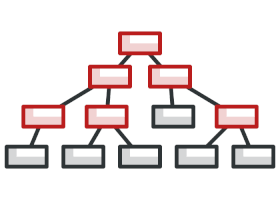
\includegraphics[width=5cm]{./imagenes/patrones.png} 
	\end{center}
\subsection{Historia}
El concepto de los patrones fue descrito por Christopher Alexander en el libro "El lenguaje de patrones" y la idea fue recogida por cuatro autores: Erich Gamma, John Vlissides, Ralph Johnson y Richard Helm. En 1995, publicaron Patrones de diseño, en el que aplicaron el concepto de los patrones de diseño a la programación.\\ El libro presentaba 23 patrones que resolvían varios problemas del diseño orientado a objetos y se convirtió en un éxito de ventas con rapidez. Al tener un título tan largo en inglés, la gente empezó a llamarlo “el libro de la ‘gang of four’ (banda de los cuatro)”, lo que pronto se abrevió a “el libro GoF”.
\begin{center}
	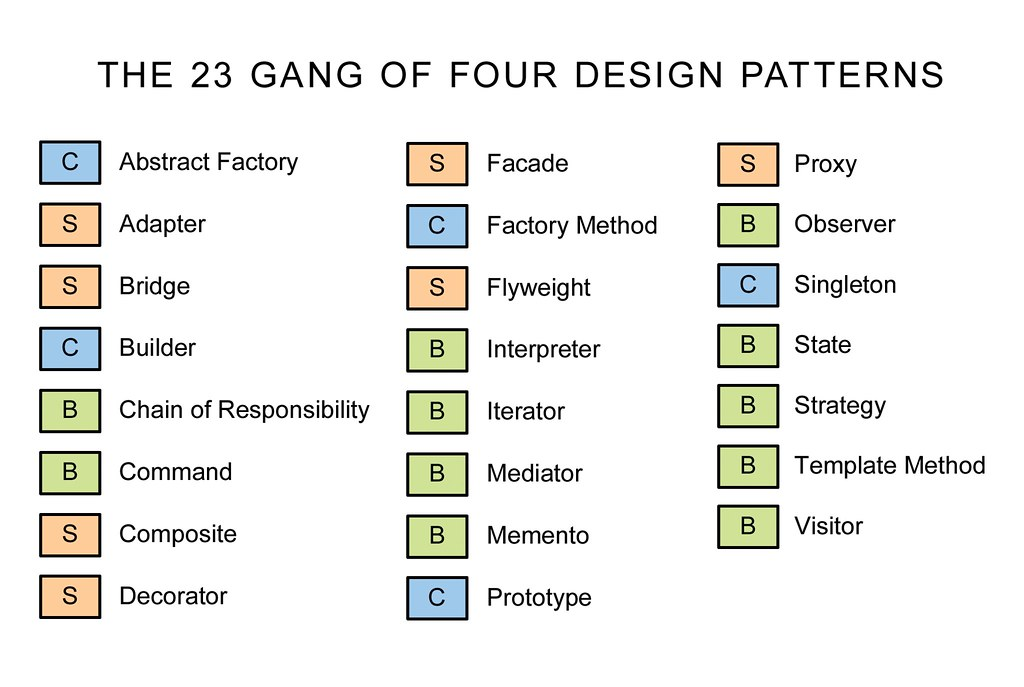
\includegraphics[width=8cm]{./imagenes/dp.jpg}
	\end{center}
\subsection{Elementos esenciales del patron}

\begin{itemize}
\item El nombre del patron.
Permite describir, en una o dos palabras, un problema de diseño junto con sus soluciones y consecuencias.
\item El problema.
Describe cuando aplicar el patron. Explica el problema y su contexto. Puede describir problemas concretos de diseño (por ejemplo: como representar algoritmos como objetos).
\item La solucion.
Describe los elementos que constituyen el diseño, sus relaciones, responsabilidades y colaboraciones. La solucion no describe un diseño o una implementacion en concreto, sino que un patron es mas bien como una plantilla que puede aplicarse en muchas situaciones diferentes. El patron proporciona una descripcion abstracta de un problema de diseño y como lo resuelve una disposicion general de elementos (en nuestro caso, clases y objetos).
\item Las consecuencias.
Son los resultados asi como las ventajas e inconvenientes de aplicar el patron. Aunque cuando se describen decisiones de diseño muchas veces no se reflejan sus consecuencias, estas son fundamentales para evaluar alternativas de diseño y comprender los costes y beneficios de aplicar el patron.
\end{itemize} 
\subsection{¿Como resuelven los patrones los problemas de diseño?}
\\Encuentran los módulos apropiados.
\\Determinan la granularidad de los módulos: Establecen el nivel de abstracción adecuado para representar componentes del sistema.
\\Especificar las interfaces de los módulos: Establecen relaciones de herencia, composición y signatura de métodos que aparecen en la interfaz de los módulos.
\subsection{¿Como seleccionar un patron de diseño?}
\\• Considerar los problemas que resuelve cada patrón
\\• Prestar atención al propósito de cada patrón y a toda su documentación.
\\• Estudiar como se interrelacionan los patrones
\\• Analizar patrones de propósito general
\\• Examine los item de cambio
\\• Piense en qué aspectos querrá modicar el diseño a futuro (ampliaciones/reducciones del sistema)
\subsection{¿Que debe tener un patron de diseño?}
\begin{center}
	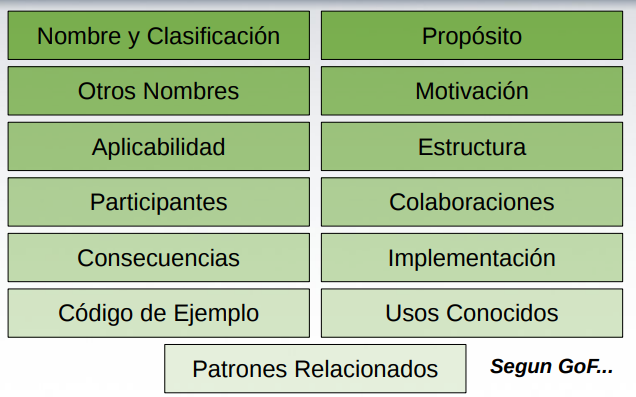
\includegraphics[width=6cm]{./imagenes/tener.png} 
	\end{center}
\subsection{¿Como usar un patron de diseño?}
\\1.Leer el patrón una vez para tener una visión general
\\2. Volver y estudiar la estructura, los participantes y las
colaboraciones
\\3. Ver un ejemplo concreto codificado del patrón
\\4. Elegir nombres para los participantes del patrón que
sean significativos en el contexto de la aplicación
\\5. Definir las clases
\\6. Definir nombres específicos de la aplicación para las operaciones en el patrón
\\7. Implementar las operaciones que realizarán las responsabilidades y colaboraciones del patrón
\subsection{Clasificacion de los patrones}
Según su propósito:\\
– De creación: conciernen al proceso de creación
de objetos.\\
– De estructura: tratan la composición de clases
y/o objetos.\\
– De comportamiento: caracterizan las formas en
las que interactúan y reparten responsabilidades
las distintas clases u objetos.
\begin{center}
    	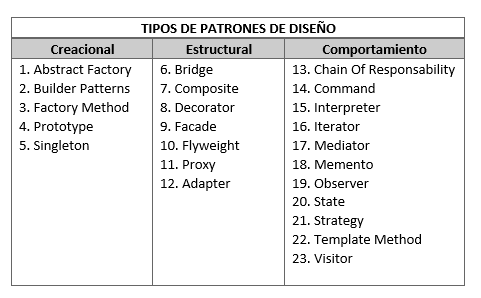
\includegraphics[width=9cm]{./imagenes/TIPOS.png} 
	\end{center}
\begin{itemize}
	\item Patrones de diseño Creacionales\\
	
 \\Abstraen el proceso de instanciación:
\\– Encapsulan el conocimiento acerca de que clase
concreta se usa
\\– Esconde como las instancias de estas clases son
creadas y unidas
\\- Da gran cantidad de flexibilidad en que se crea,
quien lo crea, como es creado, y cuando es
creado.
\\- Una patrón de clase creacional usa la herencia
para variar la clase que es instanciada
\\- Un patrón de objeto creacional delega la
instanciación a otro objeto.
\\\\Los patrones creacionales más conocidos son:

\\- Abstract Factory: Nos provee una interfaz que delega la creación de un conjunto de objetos relacionados sin necesidad de especificar en ningún momento cuáles son las implementaciones concretas.
\\- Factory Method: Expone un método de creación,  delegando en las subclases la implementación de este método.
\\- Builder: Separa la creación de un objeto complejo de su estructura, de tal forma que el mismo proceso de construcción nos puede servir para crear representaciones diferentes.
\\- Singleton: limita a uno el número de instancias posibles de una clase en nuestro programa, y proporciona un acceso global al mismo.
	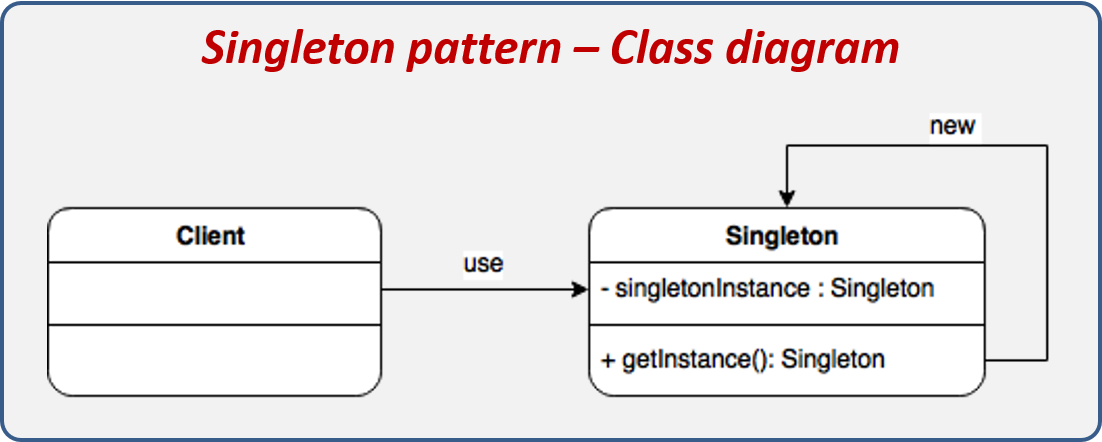
\includegraphics[width=6cm]{./imagenes/creacion.png}\\
	
\\- Prototype: Permite la creación de objetos basados en “plantillas”. Un nuevo objeto se crea a partir de la clonación de otro objeto.

	\item Patrones de diseño Estructural

\\Los patrones de diseño estructurales se preocupan de
como las clases y objetos se unen para formar
estructuras más grandes.
\\- Un patrón de clase estructural usa la herencia para componer interfaces o implementación; la composición es fijada en tiempo de diseño
\\- Un patrón de objeto estructural describe la manera de componer los objetos para crear nueva funcionalidad;
la flexibilidad añadida a la composición de objetos
viene de la agilidad de cambiar la composición en
tiempo de ejecución\\
\\Estos son los patrones estructurales que definió la Gang of Four:

\\- Adapter: Permite a dos clases con diferentes interfaces trabajar entre ellas, a través de un objeto intermedio con el que se comunican e interactúan.
\\- Bridge: Desacopla una abstracción de su implementación, para que las dos puedan evolucionar de forma independiente.
\\- Composite: Facilita la creación de estructuras de objetos en árbol, donde todos los elementos emplean una misma interfaz. Cada uno de ellos puede a su vez contener un listado de esos objetos, o ser el último de esa rama.
	\begin{center}
	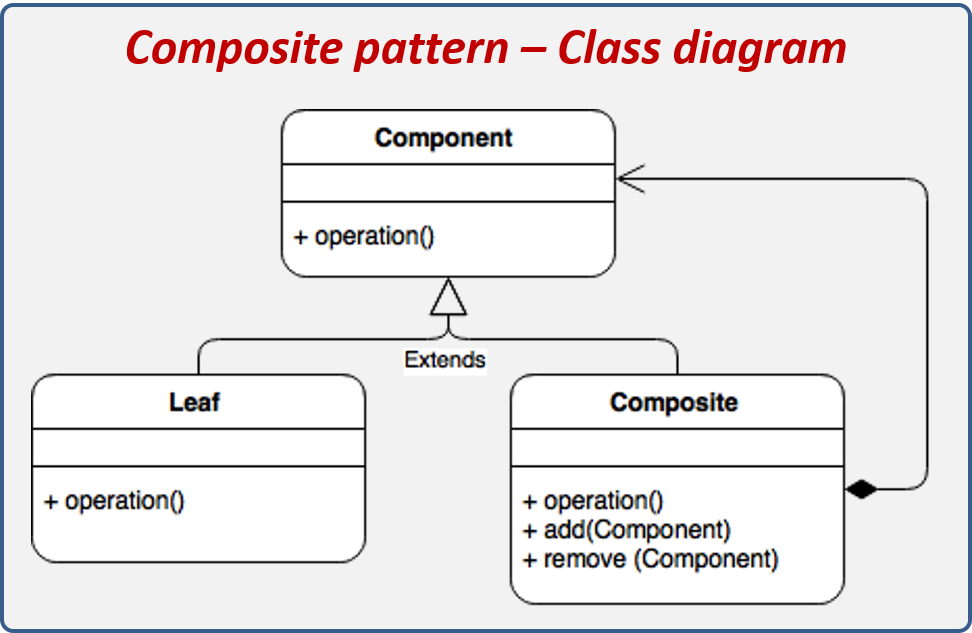
\includegraphics[width=6cm]{./imagenes/est.png} 
	\end{center}
\\- Decorator: Permite añadir funcionalidad extra a un objeto (de forma dinámica o estática) sin modificar el comportamiento del resto de objetos del mismo tipo.
\\- Facade: Una facade (o fachada) es un objeto que crea una interfaz simplificada para tratar con otra parte del código más compleja, de tal forma que simplifica y aísla su uso. Un ejemplo podría ser crear una fachada para tratar con una clase de una librería externa.
\\- Flyweight: Una gran cantidad de objetos comparte un mismo objeto con propiedades comunes con el fin de ahorrar memoria.
\\- Proxy: Es una clase que funciona como interfaz hacia cualquier otra cosa: una conexión a Internet, un archivo en disco o cualquier otro recurso que sea costoso o imposible de duplicar.
	\item Patrones de diseño de comportamiento
	Los patrones de diseño de comportamiento se
preocupan acerca de los algoritmos y de la asignación
de responsabilidades entre los objetos.
	\\- Los patrones de clase de comportamiento usan herencia para distribuir el comportamiento entre las
clases
	\\- Los patrones de objeto de comportamiento usan la composición de objetos en vez de la herencia.; algunos
describen como un grupo de objetos coopera para
llevar a cabo una tarea que un objeto simple no puede ejecutar por si mismo; otros tratan acerca de la encapsulación de comportamiento en un objeto y la delegación de peticiones a él.\\
Los patrones de comportamiento son:

\\- Command: Son objetos que encapsulan una acción y los parámetros que necesitan para ejecutarse.
\\- Chain of responsibility: se evita acoplar al emisor y receptor de una petición dando la posibilidad a varios receptores de consumirlo. Cada receptor tiene la opción de consumir esa petición o pasárselo al siguiente dentro de la cadena.
\\- Interpreter: Define una representación para una gramática así como el mecanismo para evaluarla. El árbol de sintaxis del lenguaje se suele modelar mediante el patrón Composite.
\\- Iterator: Se utiliza para poder movernos por los elementos de un conjunto de forma secuencial sin necesidad de exponer su implementación específica.
\\- Mediator: Objeto que encapsula cómo otro conjunto de objetos interactúan y se comunican entre sí.
\\- Memento: Este patrón otorga la capacidad de restaurar un objeto a un estado anterior
\\- Observer: Los objetos son capaces de suscribirse a una serie de eventos que otro objetivo va a emitir, y serán avisados cuando esto ocurra.
\\- State: Permite modificar la forma en que un objeto se comporta en tiempo de ejecución, basándose en su estado interno.
\\- Strategy: Permite la selección del algoritmo que ejecuta cierta acción en tiempo de ejecución.
Template Method: Especifica el esqueleto de un algoritmo, permitiendo a las subclases definir cómo implementan el comportamiento real.
\\- Visitor: Permite separar el algoritmo de la estructura de datos que se utilizará para ejecutarlo. De esta forma se pueden añadir nuevas operaciones a estas estructuras sin necesidad de modificarlas.
	\begin{center}
	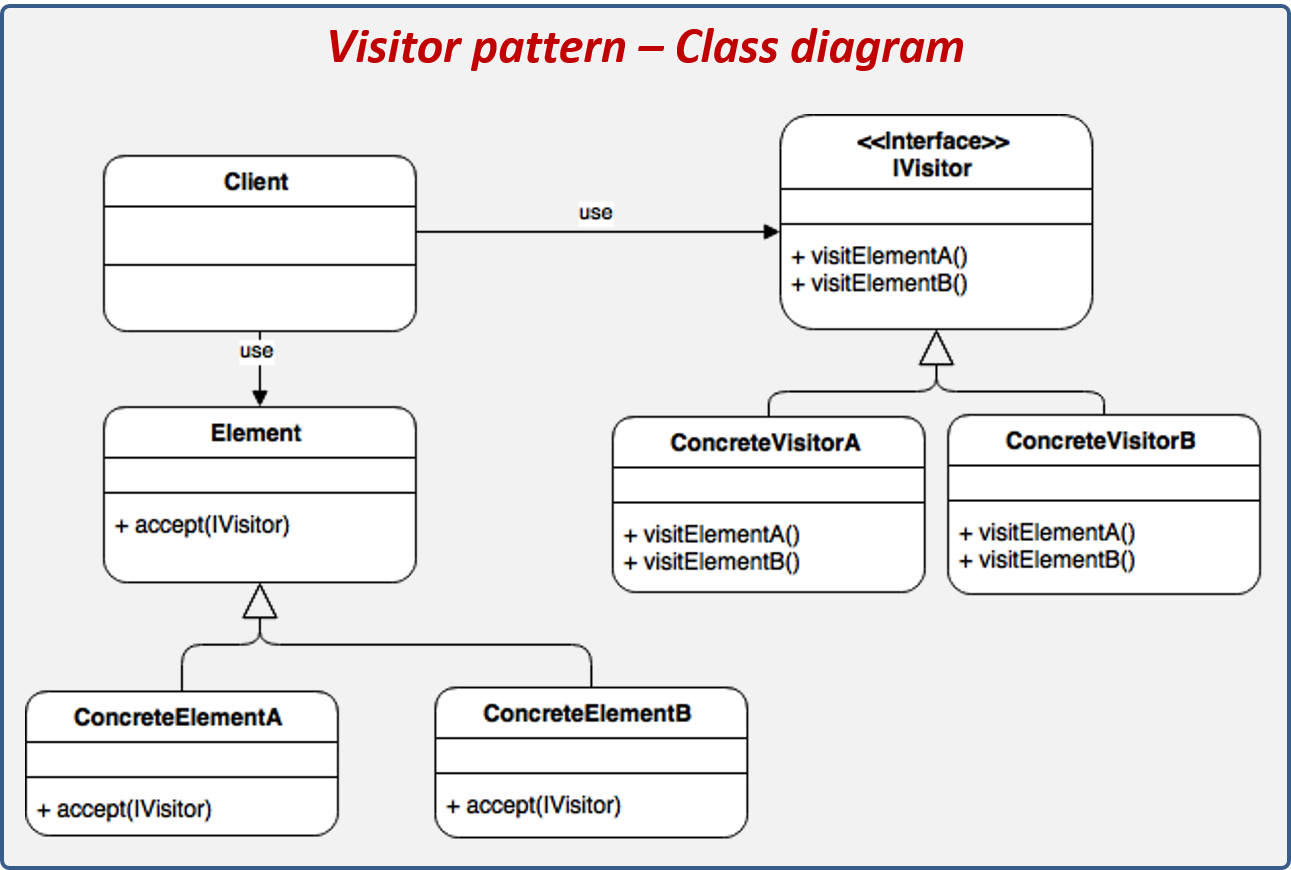
\includegraphics[width=6cm]{./imagenes/comp.png} 
	\end{center}
\end{itemize} 
\section{Conclusiones}

La conclusion es sencilla, si no usas patrones, deberias hacerlo. Los patrones ayudan a estandarizar el codigo, haciendo que el diseño sea mas comprensible para otros programadores. Son muy buenas herramientas, y siempre deberiamos usar las mejores herramientas a nuestro alcance. Los patrones de diseño nos permiten tener una mejor estructura de software. El uso de patrones ayuda a obtener un software de calidad (extensibilidad y reutilizacion).

\section{Recomendaciones}
Se recomienda no abusar de los patrones de diseño: no intentes usar un patron de diseño solo porque lo conoces, te puede complicar mas que ayudar. Los patrones dediseño son una plantilla de soluciones, los puedes usar adaptandolos a tu problema particular. Pero respeta siempre el concepto sobre el que descansa, si tienes que modificar demasiadas cosas de un patron para que se adapte a tu problema, quizas sea mejor no utilizarlo.
%----------------------------------------------------------------------------------------
%	REFERENCE LIST
%----------------------------------------------------------------------------------------

\begin{thebibliography}{99} % Bibliography - this is intentionally simple in this template
Freeman, E. Sierra, K. Bates, B. (2004) Head first design patterns
\url{http://ce.sharif.edu/courses/98-99/2/ce484-1/resources/root/Design%20Patterns/Eric%20Freeman,%20Elisabeth%20Freeman,%20Kathy%20Sierra,%20Bert%20Bates-Head%20First%20Design%20Patterns%20-OReilly%20(2008).pdf} 
\\ \\ Ecotec (s.f.) Programacion Orientada a objetos: Patrones de diseño
\url{https://www.ecotec.edu.ec/documentacion/investigaciones/docentes_y_directivos/articulos/6068_TRECALDE_00288.pdf} \\ \\ 
Pavon, J. (2004) Patrones de diseño orientado a objetos
\url{https://www.fdi.ucm.es/profesor/jpavon/poo/2.14pdoo.pdf}
\\ \\ 
Postan, E. (2003) Patrones de diseño
\url{https://www.fceia.unr.edu.ar/ingsoft/Contribuciones/Patrones.pdf}
\\ \\
Gutierrez, D. (2010) Patrones de diseño
\url{http://www.codecompiling.net/files/slides/IS_clase_09_patrones_diseno.pdf}
\\ \\ 
Goñi, A. (S.f) Patrones de diseño
\url{http://siul02.si.ehu.es/~alfredo/iso/06Patrones.pdf}
\\ \\ 
Gamma, E. ,Helm,R. , Johnson, R. , vlissides, J. (2003) PAtrones de diseño, elementos de software orientado a objetos reutilizable
\url{https://profeuttec.yolasite.com/resources/Patrones%20de%20dise%C3%B1o%20-%20Erich%20Gamma.pdf}
\\ \\ 
Leiva,A. (2016) Los 7 patrones de diseño de software más importantes
\url{https://dev.to/gelopfalcon/los-7-patrones-de-diseno-de-software-mas-importantes-28l2}
\\ \\ 
Leiva,A. (2016) patrones de diseño de software
\url{https://devexperto.com/patrones-de-diseno-software/}
\\ \\ 
Refactoring guru (s.f.) Patrones de diseño
\url{https://refactoring.guru/es/design-patterns/java}
 \\ \\ 
 
\end{thebibliography}

%----------------------------------------------------------------------------------------

\end{document}
